%%%%%%%%%%%%%%%%%%%%%%%%%%%%%%%%%%%%%%%%%%%%%%%%%%%%%%%%%%%%%%%%%%%%%%%%%%%%
%% Trim Size : 11in x 8.5in
%% Text Area : 9.6in (include Runningheads) x 7in
%% ws-jai.tex, 26 April 2012
%% Tex file to use with ws-jai.cls written in Latex2E.
%% The content, structure, format and layout of this style file is the
%% property of World Scientific Publishing Co. Pte. Ltd.
%%%%%%%%%%%%%%%%%%%%%%%%%%%%%%%%%%%%%%%%%%%%%%%%%%%%%%%%%%%%%%%%%%%%%%%%%%%%
%%

%\documentclass[draft]{ws-jai}
\documentclass{ws-jai}
\usepackage[flushleft]{threeparttable}
\usepackage{siunitx}
\usepackage{amsmath}
\usepackage{gensymb}
\usepackage[colorlinks=true,allcolors=blue]{hyperref}
\usepackage{graphicx}
\usepackage{caption}
\usepackage{subcaption}
\usepackage[bottom]{footmisc}
\usepackage{url}



\begin{document}

\catchline{}{}{}{}{} % Publisher's Area please ignore

\markboth{Author's Name}{Paper Title}

\title{Instructions for Typesetting Manuscript\\
Using \LaTeX\footnote{For the title, try not to use more than
three lines. Typeset the title in 11 pt Times Roman,
boldface, with the first letter of important words capitalized.}}

\author{First Author$^{2}$, Second Author$^{3}$, Third Author$^{3}$ and Fourth Author$^{4}$}

\address{
$^{2}$Department, University Name, City, State ZIP/Zone, Country, fauthor@university.com\\
$^{3}$Group, Company, Address, City, State ZIP/Zone, Country\\
$^{4}$Group, Company, Address, City, State ZIP/Zone, Country, fauthor@company.com
}

\maketitle

\corres{$^{2}$Corresponding author.}

\begin{history}
\received{(to be inserted by publisher)};
\revised{(to be inserted by publisher)};
\accepted{(to be inserted by publisher)};
\end{history}

\begin{abstract}
The low frequency radio astronomy has the highest potential in discovering the history of the Universe, this includes observations of the first stars and the mapping of dark ages. The Array of Long Baseline Antennas for Taking Radio Observations from the Sub-Antarctic (ALBATROS) is a new interferometric array. It consists of autonomous antenna stations that will map the low-frequency sky from Marion Island. One autonomous station was deployed in Marion Island in April 2019. The operating frequency range is \SIrange{1.2}{81}{\MHz} with baselines of $\approx \SI{20}{\km}$. A two element inteferometer, the ALBATROS - Exploratory Gizmo on the Ground (ALBATROS-EGG) was deployed in Marion Island in April 2018. \\
\end{abstract}

\keywords{Keyword 1; keyword 2; keyword 3.}

\section{Introduction}
\noindent The \SI{21}{\cm} wavelength of hydrogen gas is being observed by several experiments which are modelled for the purpose of Hydrogen mapping in our Universe. This hydrogen line is a significant mechanism as it helps in the probing of the dark ages to the epoch of reionization (EoR) \cite{2013PhRvD..87d3002L,2014ApJ...782...66P}.\\

Comprehensive reviews of experimental efforts exist elsewhere but none of them have made measurements at the lowest frequencies of $\lessapprox$ \SI{30}{\MHz}. This is due to the challenges namely, the ionospheric effects, radio frequency intereference (RFI), Galactic emission and instrumental systematics which is non transparent below \SI{10}{\MHz} \cite{2019JAI.....850004P}. Two of these experiments represent the lowest frequencies measured to date (Reber’s antenna, RAE-2), and the other two represent the highest resolutions achieved in this frequency range (DRAO, OVRO-LWA).\\

Grote Reber came up with the state of art by constructing a telescope which operated at very low frequencies between 0.52 MHz and 2.1 MHz, which had 192 dipoles. At \SI{2.1}{\MHz} it had a resolution of as low as $\approx$ 5 \degree. The key map of the sky was created by this experiment at \SI{2.1}{\MHz}. He also mentioned that his measurements were influenced by galactic emission and the ionosphere \cite{article, 1988A&A...195..372W}. The Radio Astronomoy Explorer-2 (RAE-2) have very low operating frequency ranges between \SIrange{0.025}{13}{\MHz}, it main science goal was to do radio astronomy evaluation of our Galaxy (the Milkyway), the Sun and all the planets including Earth. The resolution of this experiment is $\approx$ 10 \degree at \SI{4.7}{\MHz} \cite{1975A&A....40..365A}. Both of these experiments made very low resolution measurements.\\


The experiments which made the high resolution measurements are the  Dominion Radio Astrophysical Observatory (DRAO) \SI{22}{\MHz} telescope and the OVRO-LWA \SI{36}{\MHz} experiment. The DRAO telescope operated at \SI{22}{\MHz} and its resolution ranges between $\approx$ \SIrange{1.1}{1.7}{\degree}. Its main science goal was to measure the emission from discrete sources and to observe our Galaxy's emission from its environment \cite{1999A&AS..137....7R}. The OVRO-LWA operates at frequency ranges of 36.528 MHz and 73.152 MHz. At these frequencies it has an angular resolution of \SI{15}{\arcminute} \cite{2018AJ....156...32E}. ALBATROS aims at attempting to do high resolution measurements at a frequency of $<$20 MHz which do not yet exist.\\
	
Measurements of the radio sky at $\approx$ 100 MHz and below have the capability of unlocking the new observational window in the history of the universe. At the lowest frequencies (tens of MHz), subsequent observations may permit us to probe the cosmic "dark ages," one day, which is an epoch that is obscure to date \cite{2019arXiv190710853C, 2019arXiv190804296K}. This paper will describe a new project that aims to map the low-frequency sky from Marion island using an array of autonomous antenna stations. The final array will consist of  $\approx$ 10 antennas operating at 1.2-81 MHz with baselines up to 20 km. A two-element pathfinder was deployed in April 2018, the first autonomous station was deployed in April 2019 and there'll be discussion of the preliminary observations and upcoming hardware development plans.

\section{Overview of the Instrument}

The ALBATROS-EGG is a two element inteferometer which is making exploratory measurements at a frequency range of \SI{1.2}{MHz}- \SI{81}{MHz} separated by a baseline of \SI{110}{m} as shown in \autoref{Fig:ALBATROS-EGG}. It was deployed in Marion Island in April 2018. Its schematic is shown in \autoref{Fig:ALBATROS-EGG Schematic}. The system uses the dual polarisation dipole like antennas which are omidirectional patterned. The front end electonics (FEE) are configured in a printed circuit board (PCB) which makes it easy for them to be mounted on the supporting structure of the antennas. From the FEE PCB, a coaxial cable sends the signal through to the bias tee which extracts both the RF and the DC without any degradation. \\

The high pass and the low pass filter rejects the low frequency signals and high frequency signals respectively. The signal is then amplified by a $\approx$20 dB amplifier which then send the amplified signals to the Smart Network ADC Processor (SNAP) board which does the readouts and does a series of processing step. The raspberry pi interacts with the SNAP board for data storage.\\


\begin{figure}[h!]
	\begin{center}
		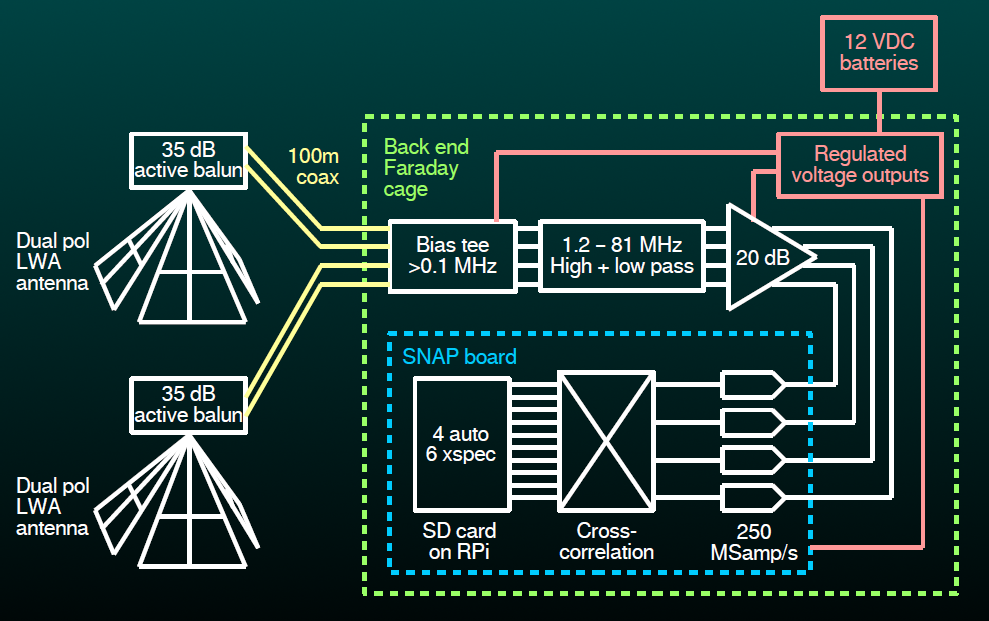
\includegraphics[width=0.55\linewidth]{Figures/ALBATROS-EGG-Schematic.PNG}
		\caption{ALBATROS - EGG pathfinder schematic which consists of the dual polarisation antennas, the 35 dB gain FEE, the 100 m coaxial cable which connects the FEE to the back end Faraday cage which comprises of the bias tee, HPF, LPF, amplifier, snap board and regulated voltage outputs which are powered by 12 VDC batteries.}
		\label{Fig:ALBATROS-EGG Schematic}
	\end{center}
\end{figure}

	\begin{figure}[h]
		\begin{center}
			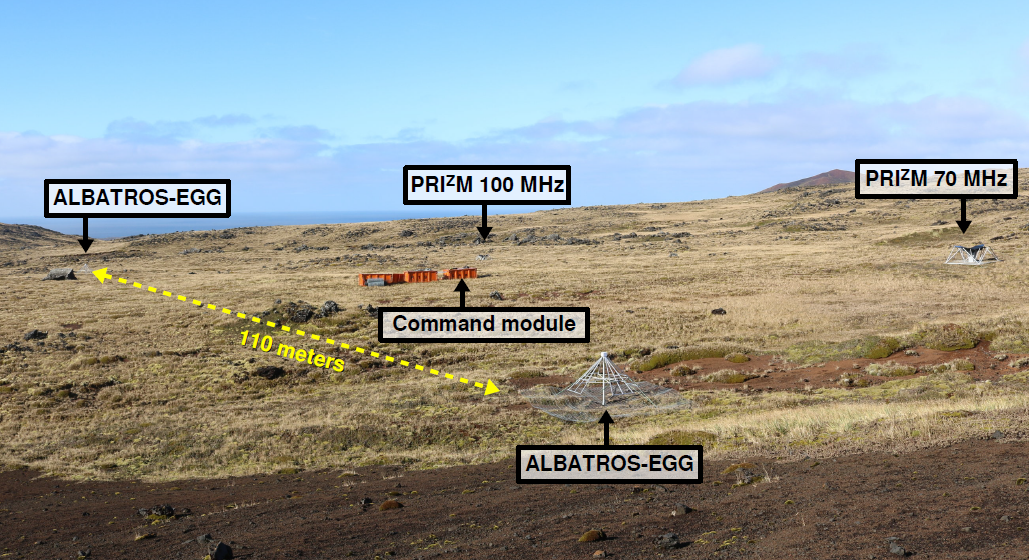
\includegraphics[width=0.7\linewidth]{Figures/ALBATROS-EGG.PNG}
			\caption{The ALBATROS-EGG pathfinder on Marion Island. The pathfinder comprises two dual-polarization antennas separated by roughly 110 m on an east-west baseline. Long coaxial cables connect the antennas to	an orange shipping container that houses the readout electronics and serves as our "command module".}
			\label{Fig:ALBATROS-EGG}
		\end{center}
	\end{figure}

The final project (ALBATROS) will consist of autonomous antenna stations that will map the low frequency sky. Since these experiments are exploratory, they are taking steps towards achieving the future objective of probing the Dark Ages.The ALBATROS stations (huts) will be separated by baselines of \SI{\approx {20}}{km} as shown in \autoref{Fig:Marion}. The two-element interferomentric pathfinder is not yet operating autonomously, it uses the direct cross correlation technique whereas the yet to be ALBATROS will write the lowest 10 - 20 MHz baseband to disk then gets correlated afterwards. One ALBATROS fully autonomous station was deployed in Marion Island in April 2019 as shown in \autoref{Fig:autonomous}. \\

The single antenna analog signal chain is shown in \autoref{Fig:Signal Chain}. The components of the system are discussed in detail as per the block diagram illustrated in \autoref{Fig:Signal Chain}. This analog signal chain is an illustration of how the first autonomous station is configured. There might be changes to the block diagram at a later stage should there be a need to revise it for the stations.

\begin{figure}[h]
	\begin{center}
		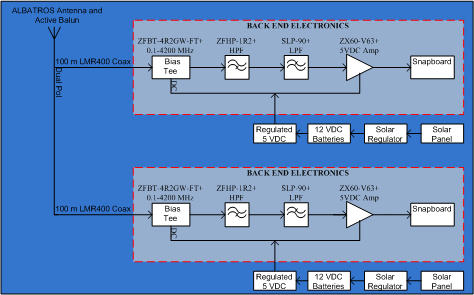
\includegraphics[width=0.7\linewidth]{Figures/Signal-Chain.png}
		\caption{Analog signal chain block diagram for the newly deployed autonomous station the ALBATROS}
		\label{Fig:Signal Chain}
	\end{center}
\end{figure}

\subsection{Antenna}	
The system uses the dual polarisation dipole like antennas which are omidirectionally patterned. The dipole like antennas are of high preference for this project because they are relatively simple and they are omnidirectionally patterned \cite{Memo28}.

\subsection{Front End Electronics (FEE)}
All the front end components were incorporated for in a double sided printed circuit board (PCB) as shown in \autoref{Fig:Balun} and the block diagram is shown in \autoref{Fig:Balun Schematic}. The Monolithic Microwave Integrated Circuits (MMICs) is the used design for the PCB. One side of the PCB is populated with components and the other side is a solid copper ground plane aperiodically stitched to the grounded copper on the side populated with components. The receiver system is made up of the active balun, filter and the gain stage that connects to the \SI{100}{\metre} coaxial cable which is connected to the back end \cite{2012PASP..124.1090H}.\\ 
The input impedance (Z\textsubscript{o}) of \SI{50}{\ohm} is introduced to the dipole by the active balun. The signal is then fed through an amplifier which amplifies it by \SI{+24}{\decibel} of gain. The balanced signal is then converted to unbalanced through a 180 \degree hybrid coupler. The band pass filter (BPF) receives the single ended signal in order for it to reject all the frequencies which are not within the range of interest. The signal gets fed to a second amplifier which again amplies it by \SI{+24}{\decibel} of gain and the output impedance of the FEE is matched to a \SI{50}{\ohm} coaxial cable. The bias tee is responsible for providing power to the FEE and extracts the RF signal by the use of the coaxial cable. This unit has an overall gain of $\approx$ \SI{35}{\decibel} and an overall noise figure of $\approx$ \SI{2.7}{\decibel} to $\approx$ \SI{2.9}{\decibel} \cite{Memo35}.

\begin{figure}[h]
	\begin{center}
		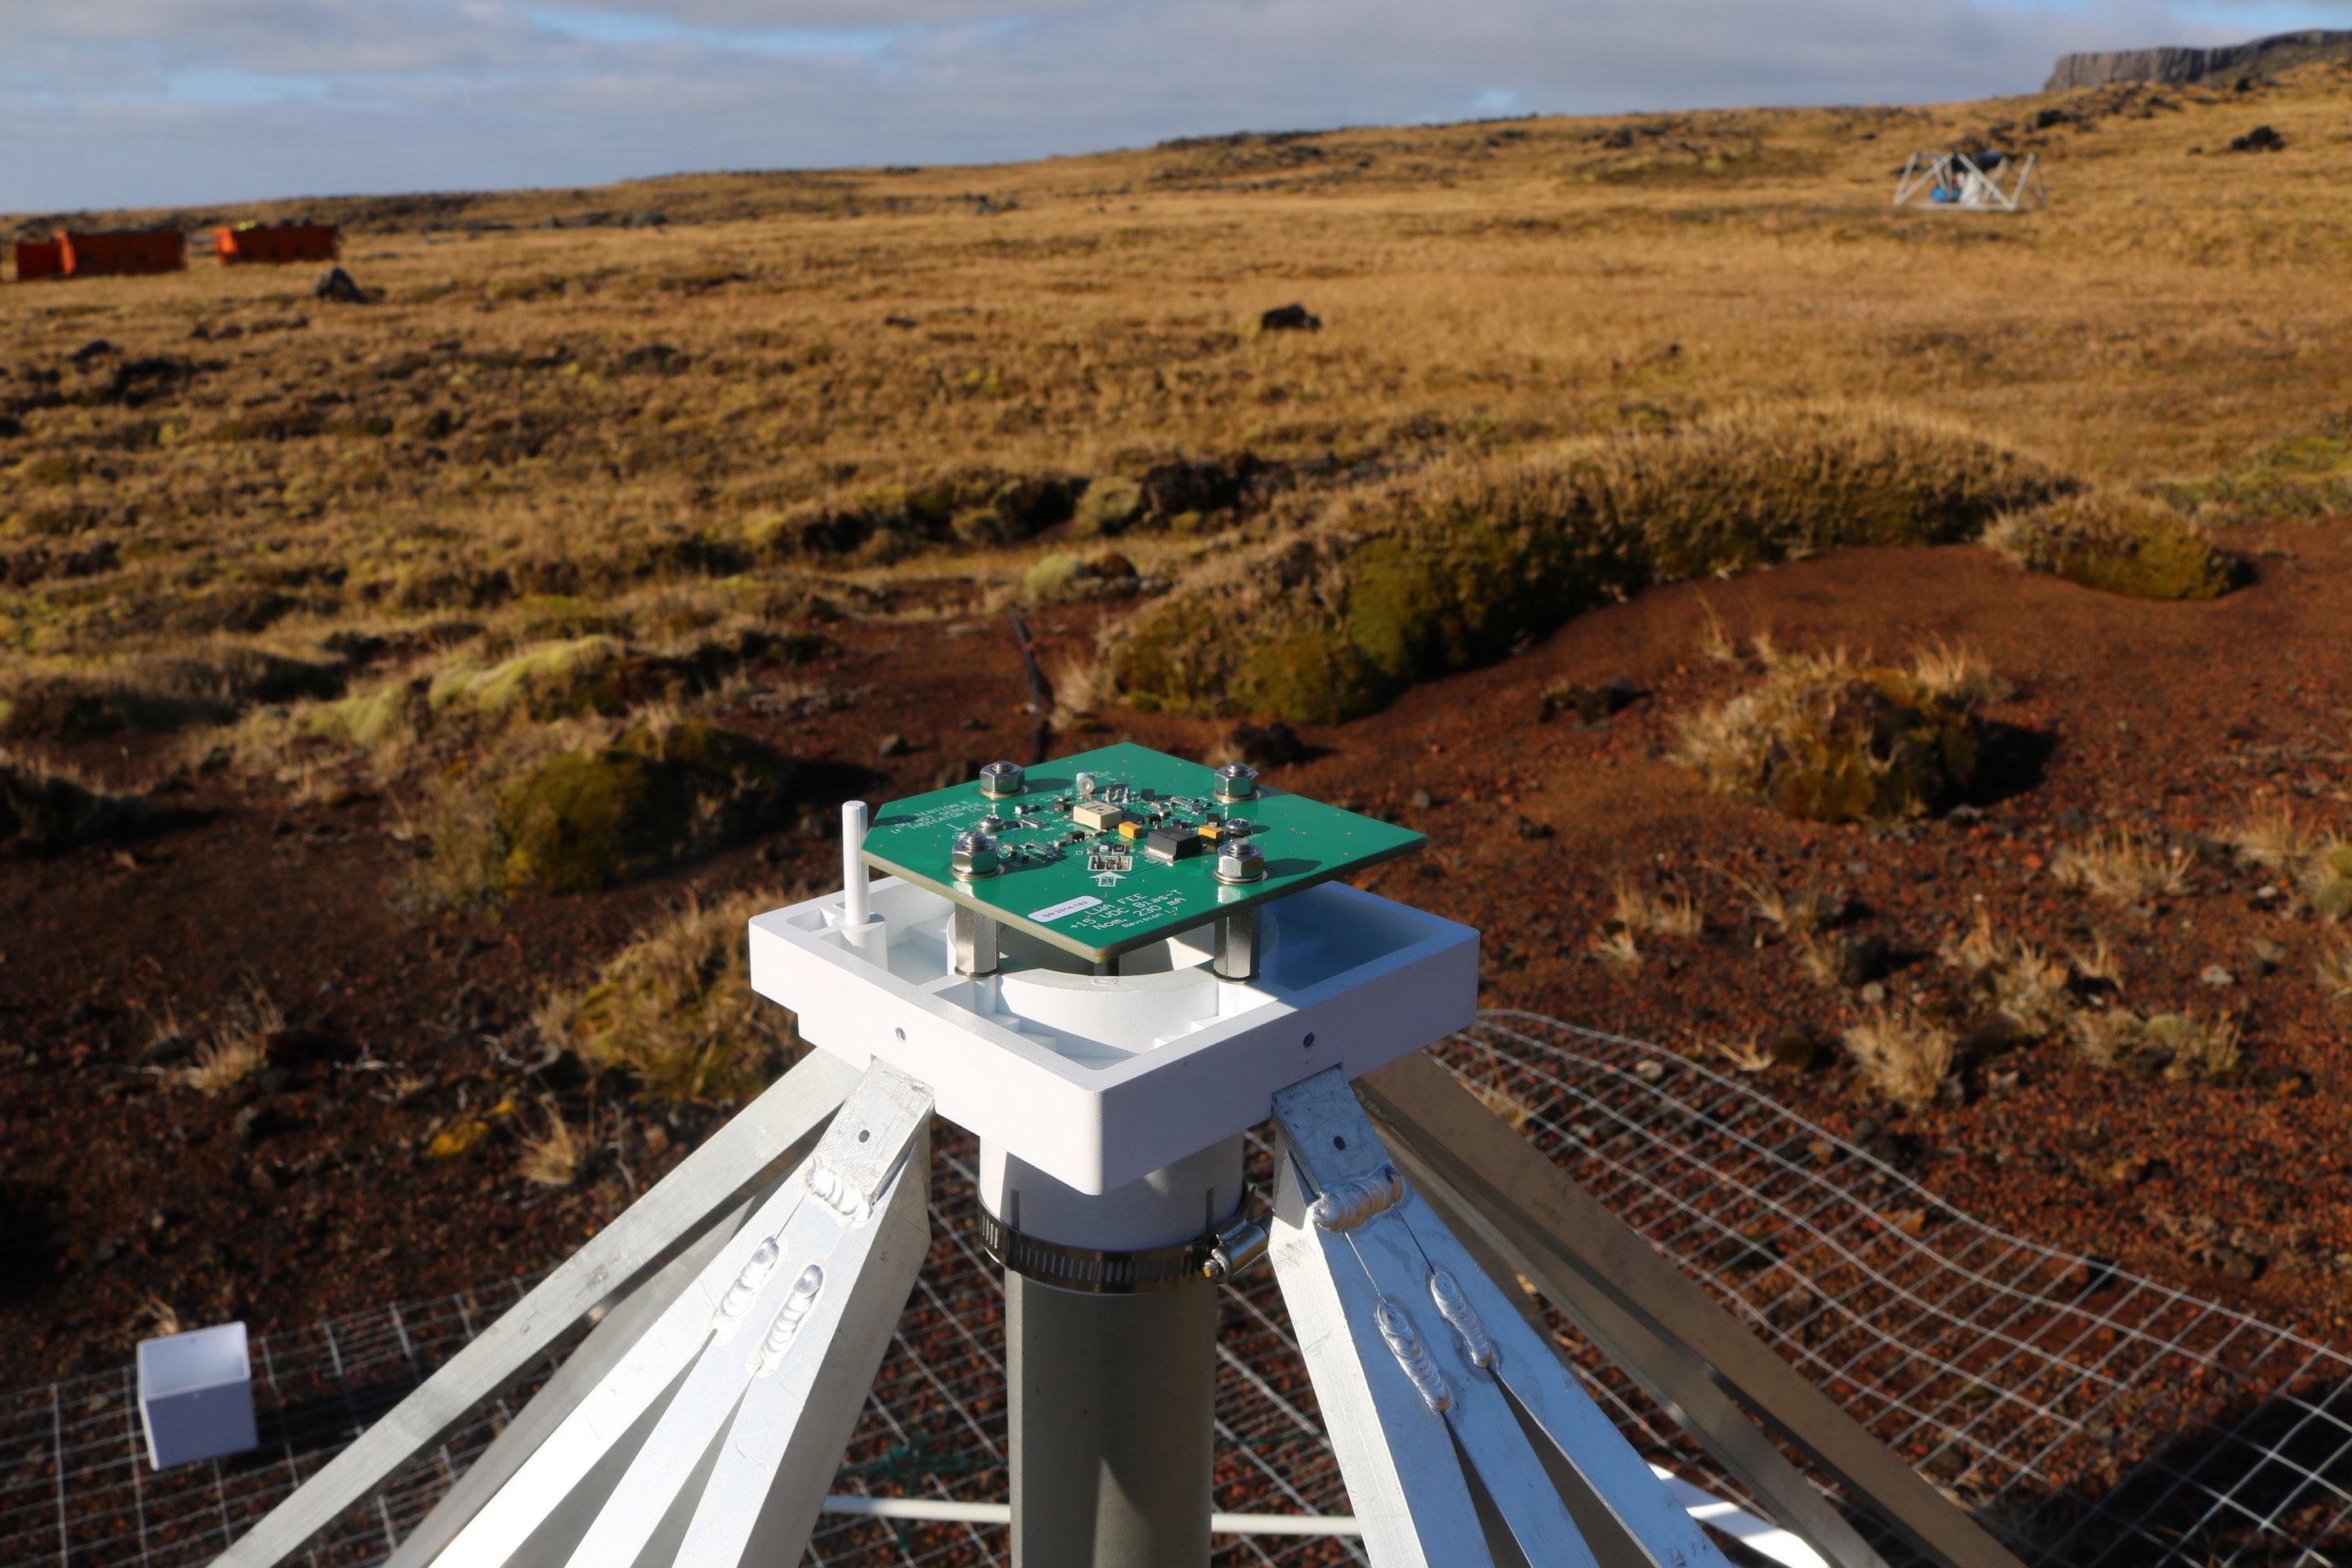
\includegraphics[width=0.5\linewidth]{Figures/balun.jpg}
		\caption{Unenclosed FEE mounted on the ALBATROS-EGG antenna supporting structure.} 
		\label{Fig:Balun}
	\end{center}
\end{figure}

\begin{figure}[h]
	\begin{center}
		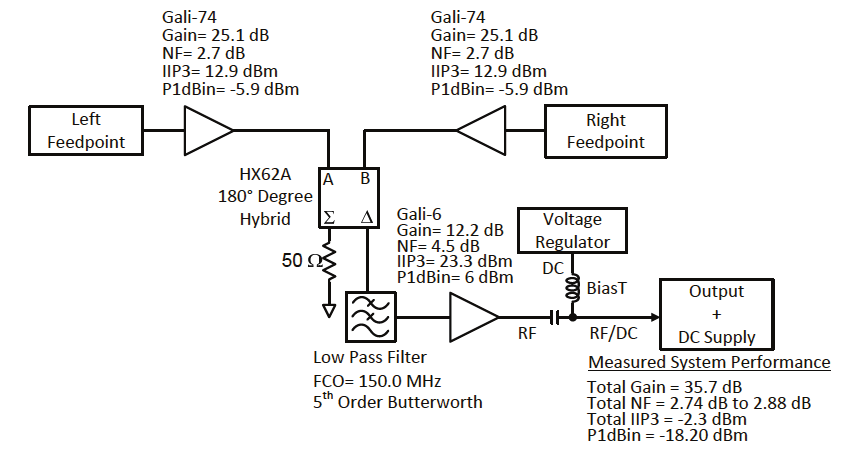
\includegraphics[width=0.7\linewidth]{Figures/Balun_Block.png}
		\caption{One Polarisation Block Diagram of the FEE \cite{2012PASP..124.1090H}}
		\label{Fig:Balun Schematic}
	\end{center}
\end{figure}

\subsection{Back End Electronics}	
The back end electronics consists of the bias tee, high pass filter (HPF), low pass filter (LPF) and the Smart Network ADC Processor (SNAP) board. \\

\textbf{Bias Tee} - It is used to extract the RF signal from a \SI{100}{\metre} LMR400 coaxial cable which has a nominal attenuation of \SI{\approx 0.4}{\decibel/\SI{100}{m}} - \SI{\approx 3.7}{dB/\SI{100}{\metre}} at \SI{1.2}{MHz} - \SI{81}{MHz} respectively \footnote{https://www.timesmicrowave.com/documents/resources/LMR-400.pdf}. The bias tee which is used is the Mini Circuits device ZFBT-4R2GW-FT+ which operates between \SI{0.14}{MHz} - \SI{4200}{MHz}. It has an insertion loss of \SI{0.16}{\decibel} at centre frequency of  \SI{\approx 10}{MHz} as per the datasheet \footnote{https://www.minicircuits.com/pdfs/ZFBT-4R2GW-FT+.pdf}.\\

\textbf{HPF} - The HPF rejects any signals with low frequencies and allow through signals with high frequencies \footnote{http://www.learningaboutelectronics.com/Articles/High-pass-filter.php}. The HPF used is the ZFHP-1R2+ Mini Circuits device which operates between  \SI{1.2}{MHz} - \SI{800}{MHz}. It has a nominal insertion loss of $\approx$ \SI{0.2}{\decibel} at centre frequency of  \SI{\approx10}{MHz} as per the datasheet \footnote{https://www.minicircuits.com/pdfs/ZFHP-1R2+.pdf}.\\

\textbf{LPF} - The LPF rejects all signals with high frequencies and allows all signals with low frequencies \footnote{http://www.learningaboutelectronics.com/Articles/Low-pass-filter.php}. The LPF used is the SLP-90+ Mini Circuits device which operates between \SI{1}{MHz} - \SI{400}{MHz}. It has a nominal insertion loss of $\approx$ \SI{0.14}{\decibel} at the centre frequency of  \SI{\approx 10}{MHz} \footnote{https://www.minicircuits.com/pdfs/SLP-90+.pdf}.\\

\textbf{Amplifier} - The amplifier at the backend amplifies the signal which is sent through to the snapboard by the gain of \SI{+20}{\decibel}. The amplifier used is the Mini Circuits device ZX60-V63+ which operates at a frequency range of \SI{0.05}{GHz} - \SI{6}{GHz}. It has a noise figure of $\approx$ \SI{3.6}{\decibel} at its lowest operating frequency of \SI{\approx 50}{MHz} \footnote{https://www.minicircuits.com/pdfs/ZX60-V63+.pdf}.\\

\textbf{SNAP Board} - The SNAP board used is specified by Xilinx Inc. \footnote{http://www.xilinx.com/products/silicon-devices/fpga/kintex-7.html}. The  SNAP board samples the signals it receives by 250 Msampl/s using internal ADCs where the signal of the clock is from the Valon 5007 frerquency synthesizer module. This creates a frequency range between \SI{0}{MHz} - \SI{125}{MHz} which contains 2048 channels. A SNAP board interacts with a raspberry pi and that is where the data is saved.\\

\subsection{Solar Power Supply System}
The power system of the ALBATROS-EGG uses generators to charge the batteries manually every once in a number of days. From the observation that has been made, the batteries take $\approx$ 2 days to discharge to a point where the system shuts down. Because of the weather conditions in Marion Island, an individual can sometimes be unable to go to the site to charge the batteries, which means that if the weather does not allow, the system can be shut down for a long period. Thus, a solar power system solution was introduced to the ALBATROS so that the system can continously run without having to be recharged manually and often.\\

The ALBATROS system is powered using \SI{24}{\volt} power which is stored and provided by two series-connected \SI{12}{\volt} deep-cycle lead-acid storage batteries. This power comes from the solar panel array consisting of nine flexible solar panels, each with a standard test condition capacity of \SI{110}{\watt}. The solar panel type is SunPower SPE-E-Flex-110. The panels are grouped in three parallel connected strings of three panels. Each group of three is mounted on its own structure. The panels include diodes to bypass shaded or defective cells, and also to prevent backwards current flow in the event an entire string of three panels is not illuminated while the others are producing power. \\

The Victron BlueSolar MPPT 50$\vert$35 charge controller outputs a data packet every second, to an Arduino based data logger, which controls a switch that determines when the rest of the system runs. It also converts the solar panel voltage to \SI{24}{\volt} to control the battery charging. The observed parameters are then stored to the raspberry pi.

\section{Pathfinder Installations and Preliminary Observations}
\subsection{Marion Island}
 Marion Island is a research location managed by the South African National Antarctic Programme (SANAP) and is located at \ang{46;54;45}S, \ang{37;44;37}E on the sub-antarctic of the Southern Indian Ocean. It is $\approx$\SI{2000}{\kilo\metre} from the nearest continental landmass which is also an approximate maximum distance for meteor scattering. The island has an area of \SI{290}{\kilo\metre\squared} and is only accessible once in April of every year by means of the S. A. Agulhas vessel owned by the Department of Environmental Affairs.  
 
 \subsection{Experiments}
 The ALBATROS-EGG shown in \autoref{Fig:ALBATROS-EGG} was installed on the PRI\textsuperscript{z}M \cite{2019JAI.....850004P} site which is located at \ang{46;53;13}S, \ang{37;49;10.7}E and the first ALBATROS station shown in \autoref{Fig:autonomous} is located \ang{46;52.205;}S, \ang{37;50.612;}E.\\
 

	\begin{figure}[h]
		\begin{center}
			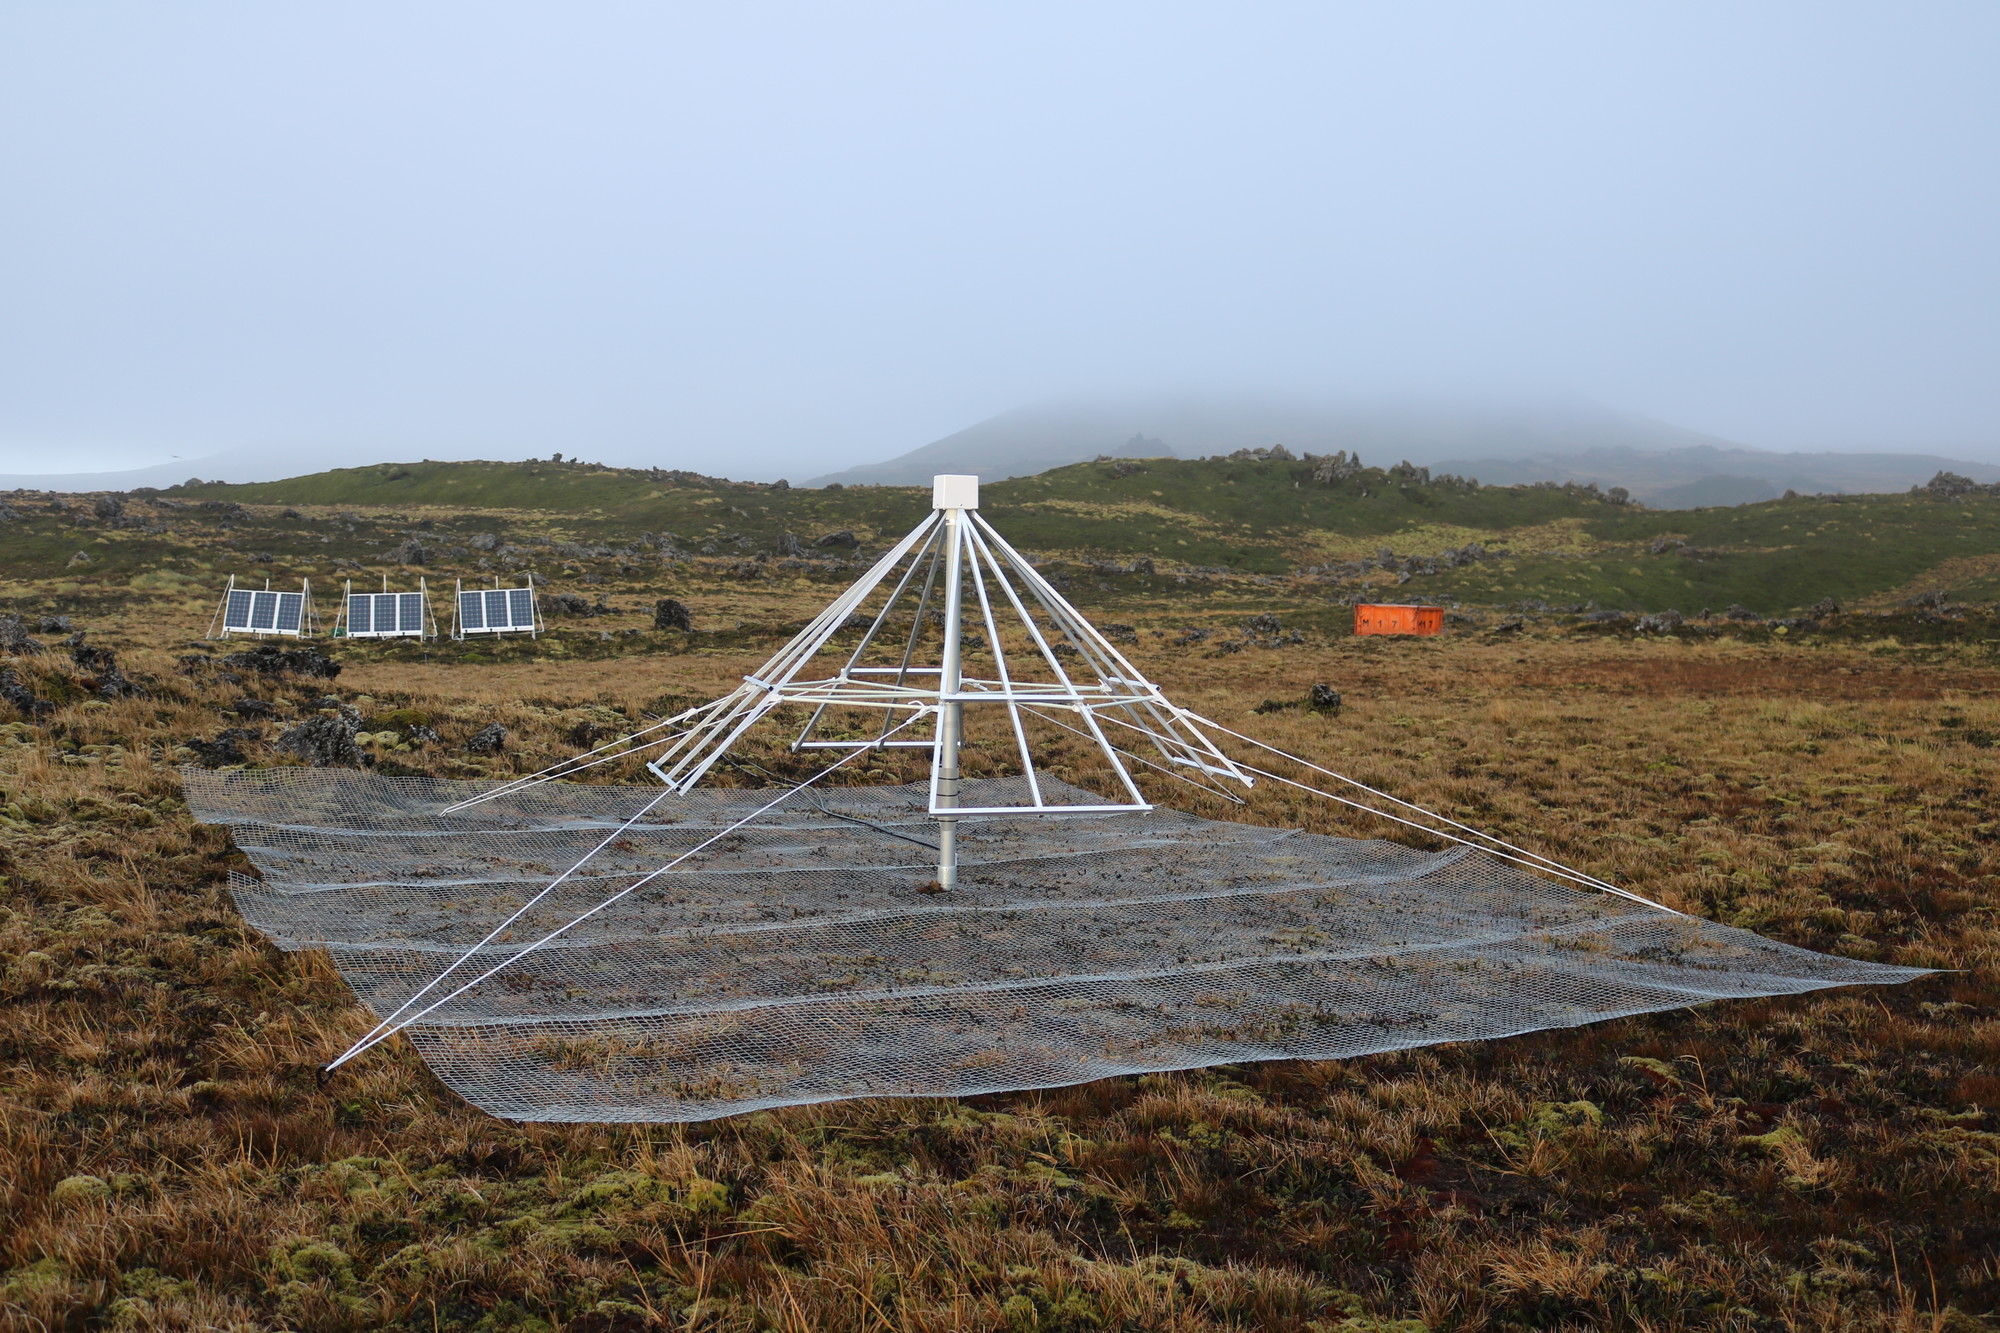
\includegraphics[width=0.7\linewidth]{Figures/autonomous.jpg}
			\caption{}
			\label{Fig:autonomous}
		\end{center}
	\end{figure}

 \subsection{Preliminary Observations}
	
\autoref{Fig:auto} and \autoref{Fig:fringes} shows the initial results from the two interferometric array. These results are an encouraging factor to proceed with the development of the autonomous stations.\autoref{Fig:auto} shows the raw ALBATROS-EGG autospectra which where the waterfall plot was taken from one polarization (pol0) over an interval of 3 days. The Galaxy rising/setting is clearly visible in the structure. There are also ripples in frequency because of uncalibrated data, and the ripples arise from reflections in the cables. There is a qualitative difference between daytime and nighttime data and this shows that the contamination from shortwave radio drops off significantly at night, when the ionosphere becomes quieter.

\begin{figure}[h!]
	\begin{center}
		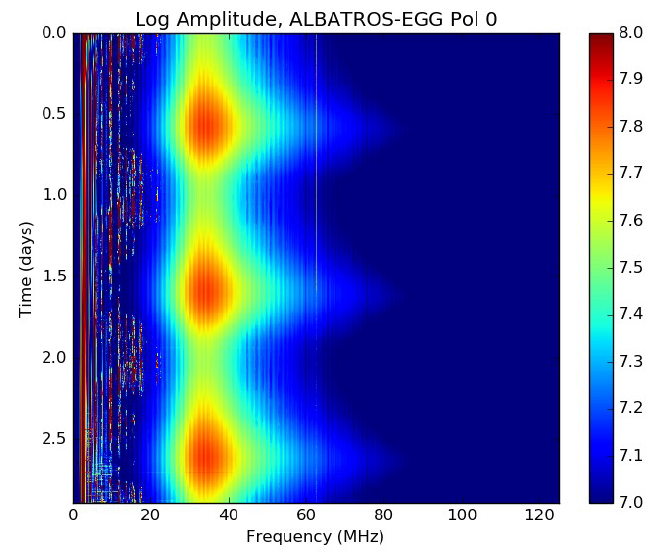
\includegraphics[width=0.8\linewidth]{Figures/Raw-ALBATROS-autospectra.PNG}
		\caption{Raw ALBATROS-EGG Autospectra}
		\label{Fig:auto}
	\end{center}
\end{figure}

\autoref{Fig:fringes} shows the first fringes that were detected by the the ALBATROS-EGG. It is dinstictly visible from \autoref{Fig:fringes} that fringes show recurrent structure down to a frequency of as low as 10 MHz without data processing or data cuts.

\begin{figure}[ht!]
	\begin{center}
		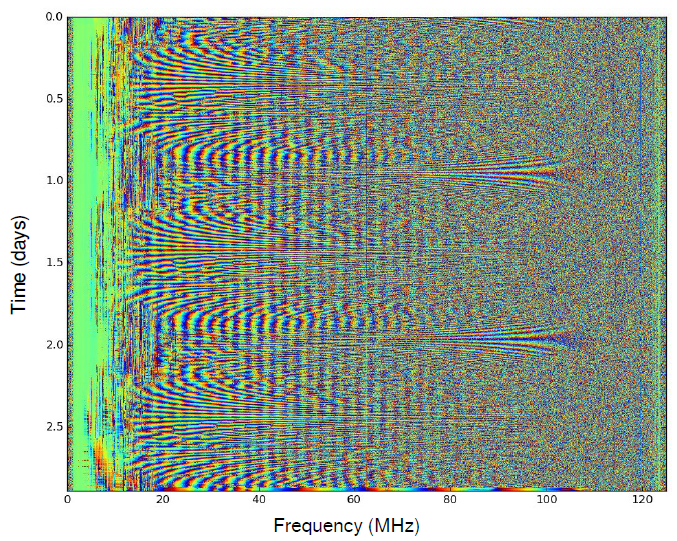
\includegraphics[width=0.7\linewidth]{Figures/First-fringes-of-ALBATROS-EGG.PNG}
		\caption{First Fringes from ALBATROS-EGG}
		\label{Fig:fringes}
	\end{center}
\end{figure}


		
\section{Future Work}

Marion Island huts which are potential stations for the ALBATROS have a ring-like pattern which is appropriate for imaging and produces a FWHM synthesized beam of 8' at 5 MHz as shown in \autoref{Fig:10}. This beam is a notable advancement over existing measurements to date.The ALBATROS main goal thus far will be to attempt to map high resolutions at low frequencies which is crucial before moving to measuring the dark ages.


\begin{figure}[h]
	\centering
	\begin{subfigure}[t]{0.5\textwidth}
		\centering
		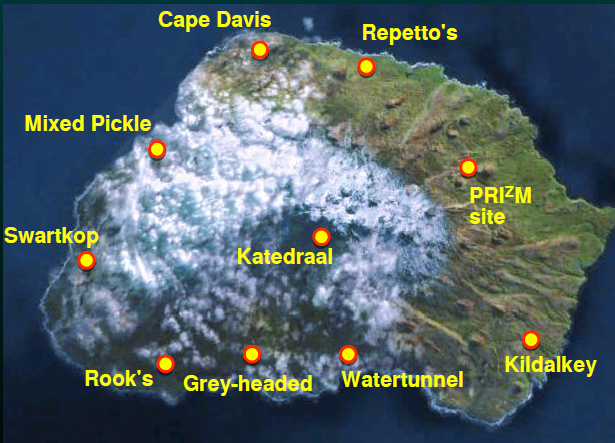
\includegraphics[width=.9\linewidth]{Figures/site.PNG}
		\caption{Marion Island huts which are potential stations for the ALBATROS. The ring-like pattern is appropriate for imaging and produces a FWHM synthesized beam of 8' at 5 MHz.}
		\label{Fig:Marion}
	\end{subfigure}%
	~~~			
	\begin{subfigure}[t]{0.5\textwidth}
		\centering
		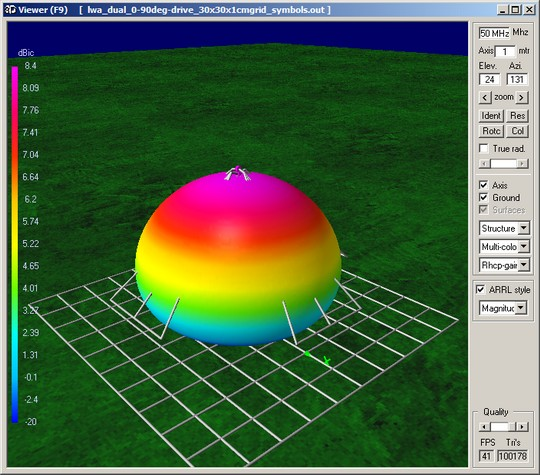
\includegraphics[width=.9\linewidth]{Figures/beam.png}
		\caption{Omnidirectional, dome shaped beam pattern which promises an improved resolution over the existing experiments to date.}
		\label{Fig:beam}
	\end{subfigure}
	\caption{Potential stations and a beam encouraging enough to implement ALBATROS experiment}
	\label{Fig:10}
\end{figure}


	
\section*{Acknowledgments}

	
\begin{thebibliography}{9}

\bibitem[Alexander et al.(1975)]{1975A&A....40..365A} Alexander, J.~K., Kaiser, M.~L., Novaco, J.~C., et al.\ 1975, {\it aap\/}, {\bf 40}, 365

\bibitem[Chen {et al.}(2019)]{2019arXiv190710853C} Chen, X., Burns, J., Koopmans, L., {\it et al.} [2019], arXiv e-prints, arXiv:1907.10853

\bibitem[Eastwood et al.(2018)]{2018AJ....156...32E} Eastwood, M.~W., Anderson, M.~M., Monroe, R.~M., et al.\ 2018, {\it aj\/}, {\bf 156}, 32

\bibitem[Ellingson and Kramer (2004)]{Memo28} Ellingson, S.~W., {Kramer}, W.~T. \ 2004, {\it Long Wavelength Array Memo (28)}

\bibitem[George {et al.}(2018)] {article} George, M., Orchiston, W., Wielebinsk, R., {\it et al.} [2018], Journal of Astronomical History and Heritage, {\bf 21}, 37

\bibitem[Hicks et al.(2012)]{2012PASP..124.1090H} Hicks, B.~C., Paravastu-Dalal, N., Stewart, K.~P., et al.\ 2012, {\it pasp\/}, {\bf 124}, 1090

\bibitem[Koopmans {et al.}(2019)]{2019arXiv190804296K} Koopmans, L., Barkana, R., Bentum, M., {\it et al.} [2019], arXiv e-prints, arXiv:1908.04296

\bibitem[Liu {et al.}(2013)]{2013PhRvD..87d3002L} Liu, A., Pritchard, J.~R., Tegmark, M., {\it et al.} [2013], {\bf 87}, 043002

\bibitem[Philip {et al.}(2019)]{2019JAI.....850004P} Philip, L., Abdurashidova, Z., Chiang, H.~C., {\it et al.} [2019], Journal of Astronomical Instrumentation, {\bf 8}, 19500

\bibitem[Pober {et al.}(2014)]{2014ApJ...782...66P} Pober, J.~C., Liu, A., Dillon, J.~S., {\it et al.} [2014], {\bf 782}, 66

\bibitem[Ray et al.(2006)]{Memo35} Ray, P.~S., Ellingson, S.~W., Fisher R., {\it et al.} [2006] {\it Long Wavelength Array Memo (35)}

\bibitem[Roger et al.(1999)]{1999A&AS..137....7R} Roger, R.~S., Costain, C.~H., Landecker, T.~L., et al.\ 1999, {\it aaps\/}, {\bf 137}, 7

\bibitem[Weiler {et al.}(1988)]{1988A&A...195..372W} Weiler, K.~W., Johnston, K.~J., Simon, R.~S., {\it et al.} [1988], {\it aap\/}, {\bf 195}, 372






\end{thebibliography}
\end{document}